% Schematic diagrams for the particle library in LevitationSim6x6.nb.
% Build:  latexmk -pdf particle_diagrams.tex   (one figure per page)
\documentclass[tikz,border=8pt]{standalone}
\usepackage{amsmath,amssymb,bm}
\usetikzlibrary{arrows.meta,calc,decorations.pathreplacing,patterns}

\tikzset{
  force/.style={-{Stealth[length=3mm]}, very thick},
  axis/.style={-{Stealth[length=2mm]}, thick},
  dim/.style={{Stealth[length=1.6mm]}-{Stealth[length=1.6mm]}, thin},
  lbl/.style={font=\small},
  note/.style={font=\footnotesize, align=left, text width=5.6cm},
  pt/.style={circle, fill, inner sep=1.4pt},
}
\definecolor{hot}{RGB}{214,69,65}
\definecolor{cold}{RGB}{52,120,196}
\definecolor{ice}{RGB}{176,214,240}
\definecolor{iceD}{RGB}{40,90,150}
\definecolor{grav}{RGB}{90,90,90}
\definecolor{thermo}{RGB}{30,140,80}

\begin{document}

%======================================================================
% 1. The harmonic thermophoretic trap
%======================================================================
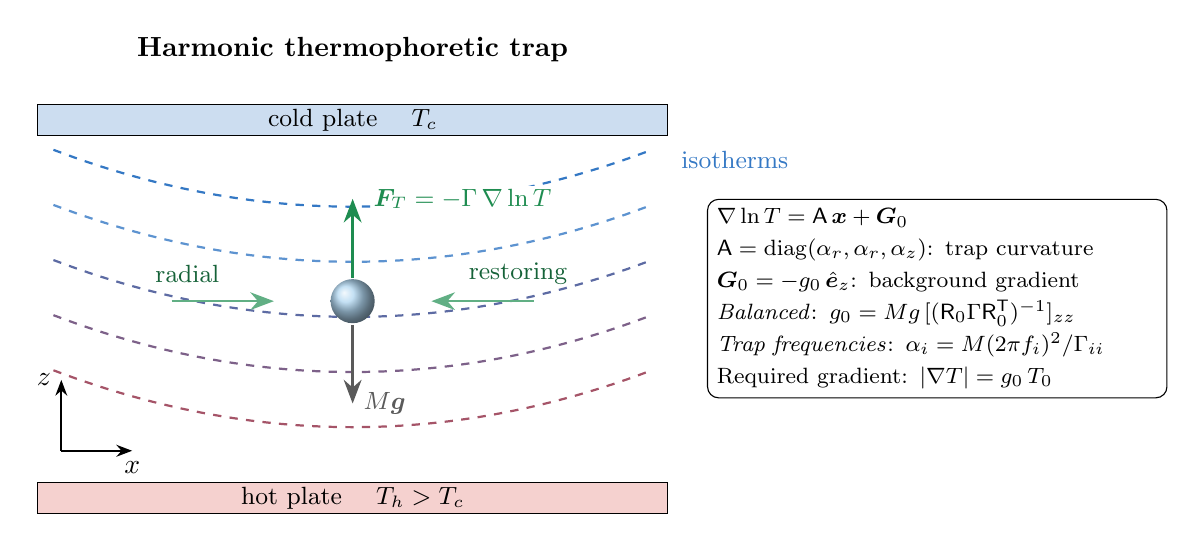
\begin{tikzpicture}[scale=1.0]
  \node[font=\bfseries] at (0,5.3) {Harmonic thermophoretic trap};
  % plates
  \fill[cold!25] (-4,4.2) rectangle (4,4.6);
  \draw (-4,4.2) rectangle (4,4.6);
  \node[lbl] at (0,4.4) {cold plate \quad $T_c$};
  \fill[hot!25] (-4,-0.6) rectangle (4,-0.2);
  \draw (-4,-0.6) rectangle (4,-0.2);
  \node[lbl] at (0,-0.4) {hot plate \quad $T_h>T_c$};
  % isotherms of ln T = alpha_r r^2/2 + alpha_z z^2/2 - g0 z  (schematic)
  \foreach \c/\col in {0.5/hot!70!cold,1.2/hot!45!cold,1.9/hot!25!cold,2.6/cold!80,3.3/cold} {
    \draw[\col, thick, dashed] plot[smooth, domain=-3.8:3.8] (\x, {\c + 0.05*\x*\x});
  }
  \node[lbl, cold, anchor=west] at (4.05,3.9) {isotherms};
  % particle and forces
  \coordinate (P) at (0,2.1);
  \shade[ball color=ice] (P) circle (0.28);
  \draw[force, thermo] ($(P)+(0,0.3)$) -- ++(0,1.0) node[right=6pt, lbl, fill=white, inner sep=1pt] {$\bm F_T=-\Gamma\,\nabla\ln T$};
  \draw[force, grav] ($(P)-(0,0.3)$) -- ++(0,-1.0) node[right, lbl] {$M\bm g$};
  % restoring arrows
  \draw[force, thermo!70, thick] (-2.3,2.1) -- (-1.0,2.1);
  \draw[force, thermo!70, thick] (2.3,2.1) -- (1.0,2.1);
  \node[lbl, thermo!70!black] at (-2.1,2.45) {radial};
  \node[lbl, thermo!70!black] at (2.1,2.45) {restoring};
  % lab axes
  \draw[axis] (-3.7,0.2) -- ++(0.9,0) node[below] {$x$};
  \draw[axis] (-3.7,0.2) -- ++(0,0.9) node[left] {$z$};
  % parameter box
  \node[note, draw, rounded corners, fill=white, anchor=north west] at (4.5,3.4) {
    $\nabla\ln T=\mathsf A\,\bm x+\bm G_0$\\[2pt]
    $\mathsf A=\mathrm{diag}(\alpha_r,\alpha_r,\alpha_z)$: trap curvature\\[2pt]
    $\bm G_0=-g_0\,\hat{\bm e}_z$: background gradient\\[2pt]
    \emph{Balanced}: $g_0=Mg\,[(\mathsf R_0\Gamma\mathsf R_0^{\mathsf T})^{-1}]_{zz}$\\[2pt]
    \emph{Trap frequencies}: $\alpha_i=M(2\pi f_i)^2/\Gamma_{ii}$\\[2pt]
    Required gradient: $|\nabla T|=g_0\,T_0$
  };
\end{tikzpicture}

%======================================================================
% 2. Sphere
%======================================================================
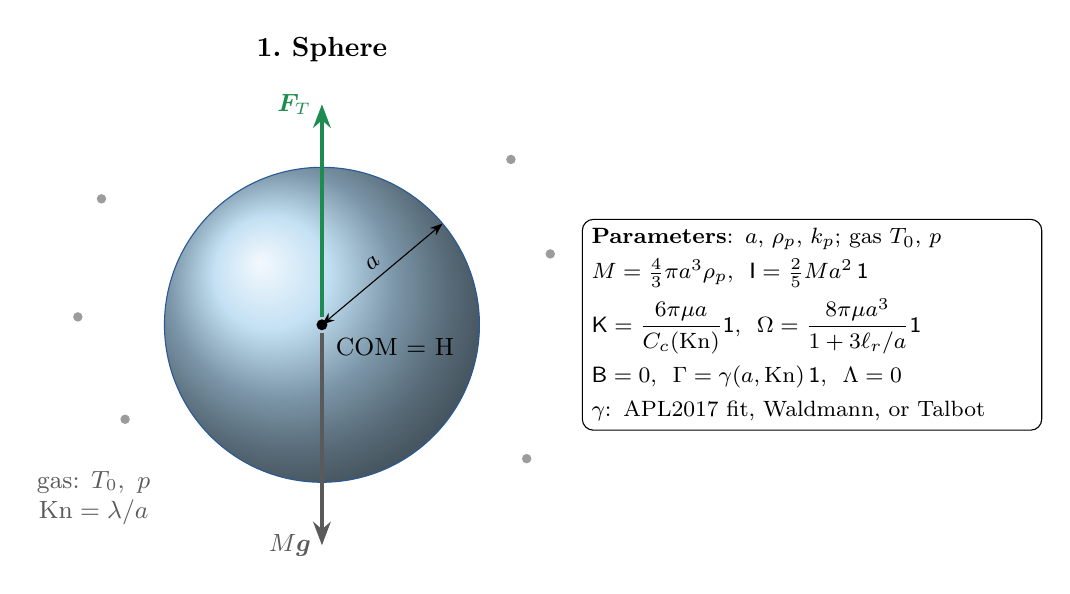
\begin{tikzpicture}[scale=1.0]
  \node[font=\bfseries] at (0,3.5) {1.\ Sphere};
  \shade[ball color=ice] (0,0) circle (2);
  \draw[iceD] (0,0) circle (2);
  \node[pt, label={[lbl]below right:COM $=$ H}] at (0,0) {};
  \draw[dim] (0,0) -- node[above, lbl, sloped] {$a$} (40:2);
  % forces
  \draw[force, thermo] (0,0.1) -- (0,2.8) node[left, lbl] {$\bm F_T$};
  \draw[force, grav] (0,-0.1) -- (0,-2.8) node[left, lbl] {$M\bm g$};
  % gas molecules
  \foreach \p in {(-2.8,1.6),(-2.5,-1.2),(2.6,-1.7),(2.9,0.9),(-3.1,0.1),(2.4,2.1)} {
    \fill[grav!60] \p circle (0.06);
  }
  \node[lbl, grav, align=center] at (-2.9,-2.2) {gas: $T_0,\ p$\\ $\mathrm{Kn}=\lambda/a$};
  \node[note, draw, rounded corners, fill=white, anchor=west] at (3.3,0) {
    \textbf{Parameters}: $a$, $\rho_p$, $k_p$; gas $T_0$, $p$\\[3pt]
    $M=\tfrac43\pi a^3\rho_p$, \ $\mathsf I=\tfrac25Ma^2\,\mathsf{1}$\\[3pt]
    $\mathsf K=\dfrac{6\pi\mu a}{C_c(\mathrm{Kn})}\mathsf{1}$, \
    $\Omega=\dfrac{8\pi\mu a^3}{1+3\ell_r/a}\mathsf{1}$\\[3pt]
    $\mathsf B=0$, \ $\Gamma=\gamma(a,\mathrm{Kn})\,\mathsf{1}$, \ $\Lambda=0$\\[3pt]
    $\gamma$: APL2017 fit, Waldmann, or Talbot
  };
\end{tikzpicture}

%======================================================================
% 3. Ellipsoid
%======================================================================
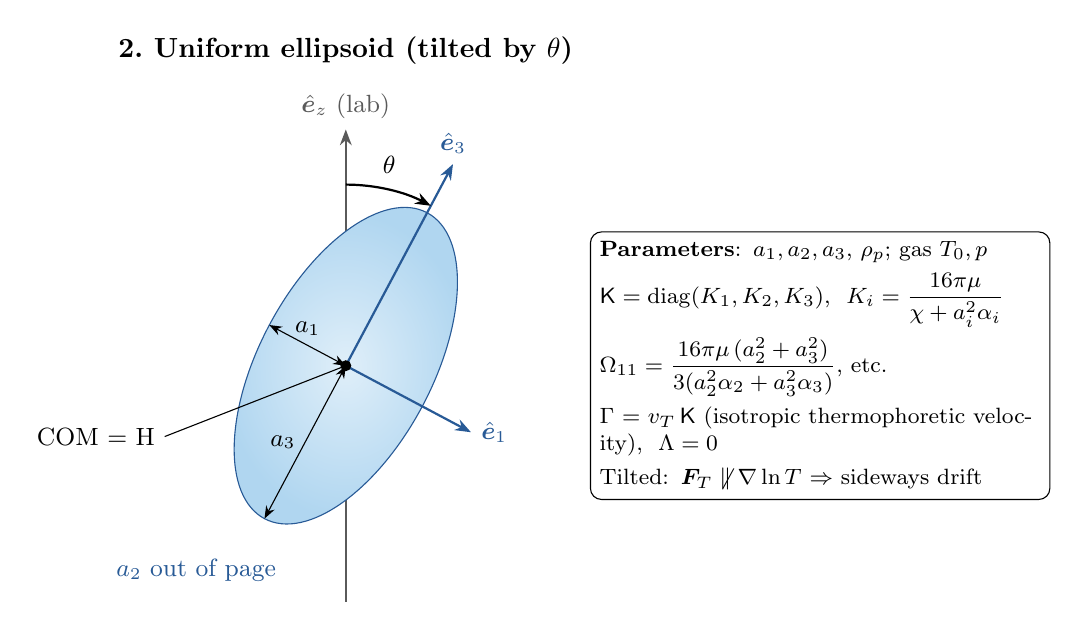
\begin{tikzpicture}[scale=1.0]
  \node[font=\bfseries] at (0,4.0) {2.\ Uniform ellipsoid (tilted by $\theta$)};
  % lab vertical
  \draw[axis, grav] (0,-3) -- (0,3) node[above, lbl] {$\hat{\bm e}_z$ (lab)};
  \begin{scope}[rotate=-28]
    \shade[inner color=ice!40, outer color=ice] (0,0) ellipse (1.1 and 2.2);
    \draw[iceD] (0,0) ellipse (1.1 and 2.2);
    \draw[axis, iceD] (0,0) -- (0,2.9) node[above, lbl] {$\hat{\bm e}_3$};
    \draw[axis, iceD] (0,0) -- (1.8,0) node[right, lbl] {$\hat{\bm e}_1$};
    \draw[dim] (0,0) -- node[left, lbl] {$a_3$} (0,-2.2);
    \draw[dim] (0,0) -- node[above, lbl] {$a_1$} (-1.1,0);
    \node[pt] at (0,0) {};
  \end{scope}
  \draw[thick, -{Stealth[length=2mm]}] (0,2.3) arc[start angle=90, end angle=62, radius=2.3];
  \node[lbl] at (0.55,2.55) {$\theta$};
  \node[lbl, iceD] at (-1.9,-2.6) {$a_2$ out of page};
  \draw[thin] (0,0) -- (-2.3,-0.9) node[left, lbl] {COM $=$ H};
  \node[note, draw, rounded corners, fill=white, anchor=west] at (3.1,0) {
    \textbf{Parameters}: $a_1,a_2,a_3$, $\rho_p$; gas $T_0,p$\\[3pt]
    $\mathsf K=\mathrm{diag}(K_1,K_2,K_3)$, \
    $K_i=\dfrac{16\pi\mu}{\chi+a_i^2\alpha_i}$\\[3pt]
    $\Omega_{11}=\dfrac{16\pi\mu\,(a_2^2+a_3^2)}{3(a_2^2\alpha_2+a_3^2\alpha_3)}$, etc.\\[3pt]
    $\Gamma=v_T\,\mathsf K$ (isotropic thermophoretic velocity), \ $\Lambda=0$\\[3pt]
    Tilted: $\bm F_T\not\parallel\nabla\ln T$ $\Rightarrow$ sideways drift
  };
\end{tikzpicture}

%======================================================================
% 4. Ellipsoid with a linear density gradient
%======================================================================
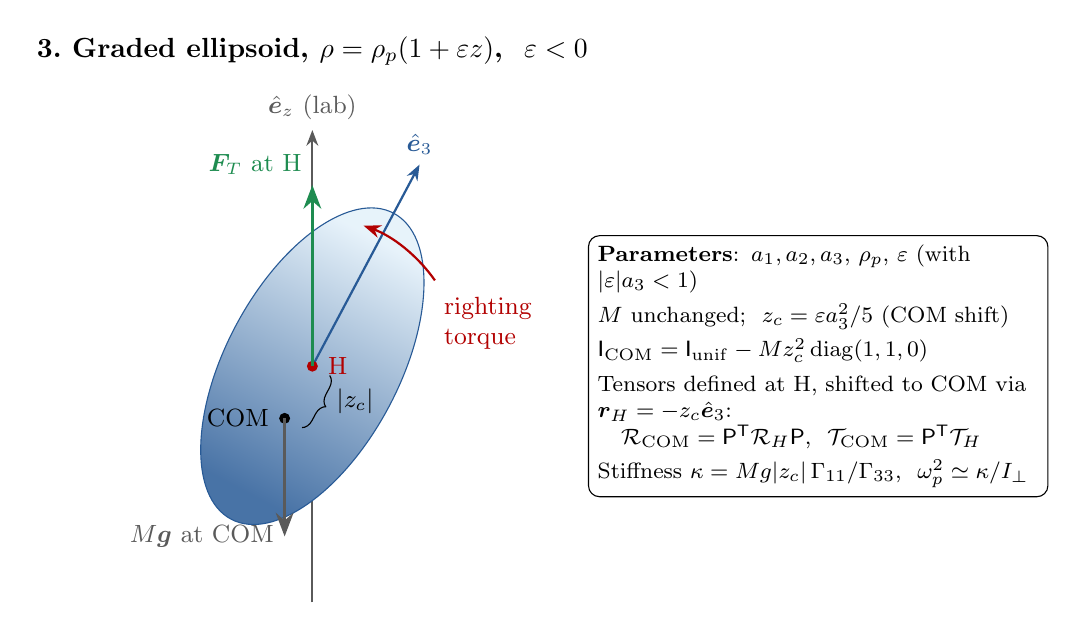
\begin{tikzpicture}[scale=1.0]
  \node[font=\bfseries] at (0,4.0) {3.\ Graded ellipsoid, $\rho=\rho_p(1+\varepsilon z)$, \ $\varepsilon<0$};
  \draw[axis, grav] (0,-3) -- (0,3) node[above, lbl] {$\hat{\bm e}_z$ (lab)};
  \begin{scope}[rotate=-28]
    % density gradient: dark (heavy) at -z end
    \shade[top color=ice!30, bottom color=iceD!85, shading angle=-28] (0,0) ellipse (1.1 and 2.2);
    \draw[iceD] (0,0) ellipse (1.1 and 2.2);
    \draw[axis, iceD] (0,0) -- (0,2.9) node[above, lbl] {$\hat{\bm e}_3$};
    \coordinate (H) at (0,0);
    \coordinate (C) at (0,-0.75);
    \node[pt, red!70!black, label={[lbl, red!70!black]right:H}] at (H) {};
    \node[pt, label={[lbl]left:COM}] at (C) {};
    \draw[decorate, decoration={brace, amplitude=4pt, mirror}] (0.25,-0.75) -- (0.25,0)
      node[midway, right=4pt, lbl] {$|z_c|$};
    % forces: F_T at H (lab vertical, drawn in lab coords below), gravity at COM
  \end{scope}
  \draw[force, thermo] (H) -- ++(0,2.3) node[above left, lbl] {$\bm F_T$ at H};
  \draw[force, grav] (C) -- ++(0,-1.5) node[left, lbl] {$M\bm g$ at COM};
  \draw[thick, -{Stealth[length=2.2mm]}, red!70!black] (35:1.9) arc[start angle=35, end angle=70, radius=1.9];
  \node[lbl, red!70!black, anchor=north west, align=left] at (1.55,1.0) {righting\\torque};
  \node[note, draw, rounded corners, fill=white, anchor=west] at (3.5,0) {
    \textbf{Parameters}: $a_1,a_2,a_3$, $\rho_p$, $\varepsilon$ (with $|\varepsilon|a_3<1$)\\[3pt]
    $M$ unchanged; \ $z_c=\varepsilon a_3^2/5$ (COM shift)\\[3pt]
    $\mathsf I_{\rm COM}=\mathsf I_{\rm unif}-Mz_c^2\,\mathrm{diag}(1,1,0)$\\[3pt]
    Tensors defined at H, shifted to COM via $\bm r_H=-z_c\hat{\bm e}_3$:\\
    \quad $\mathcal R_{\rm COM}=\mathsf P^{\mathsf T}\mathcal R_H\mathsf P$, \
    $\mathcal T_{\rm COM}=\mathsf P^{\mathsf T}\mathcal T_H$\\[3pt]
    Stiffness $\kappa=Mg|z_c|\,\Gamma_{11}/\Gamma_{33}$, \
    $\omega_p^2\simeq\kappa/I_\perp$
  };
\end{tikzpicture}

\end{document}
